\chapter{Details für Techniker}
\label{sec:details_tec}

5. Details für Techniker (meist als Anhang)
Logdateien, Bildschirmfotos, Listings, Terminalsessions, ...
Jeweils durchnummeriert, damit man darauf Bezug nehmen kann in vorherigen Teilen des Berichts
Beliebig lang

\section{Emails von Pat's PC}
\label{sec:pat_emails}

\subsection{FILE 1:}
\label{sec:pat_emails_1}

\begin{table}[htb]
	\begin{tabular}{p{2cm} p{13.5cm}}
		Name & wbk15.tmp\\
		Pfad & /img_pat_harddrive.001/Documents and Settings/Pat/Local Settings/ Temporary Internet Files/Content.IE5/6NU83K2N/wbk15.tmp\\
		Zeitstempel & 2009-11-23 17:56:33 MEZ
	\end{tabular}
\end{table}	

\begin{lstlisting}
Pat,

I understand. Don't worry - I'll take care of everything.

Terry
----- Original Message ----- 
From: Pat McGoo pat@m57.biz
To: terry t93940@gmail.com; jo@m57.biz
Sent: Friday, November 20, 2009 2:40 PM
Subject: Re: Equipment Disposal


Jo,

yes, I would be concerned about that too, thanks for thinking about 
that.

Terry - what did you /are you going to/ do with Jo's computer?

We need to make sure it is properly erased ! Thank you.

Pat
----- Original Message ----- 
From: jo@m57.biz
To: Pat McGoo pat@m57.biz
Sent: Friday, November 20, 2009 2:29 PM
Subject: Equipment Disposal


Pat,

My computer had to be swapped out today. I just want to make sure it is
properly disposed of. There could be company information on there that 
we don't want to share with the rest of the world. Right?

- Jo
\end{lstlisting}

\subsection{FILE 2:}
\label{sec:pat_emails_2}	

\begin{table}[htb]
	\begin{tabular}{p{2cm} p{13.5cm}}
		Name & wbk29.tmp\\
		Pfad & /img_pat_harddrive.001/Documents and Settings/Pat/Local Settings/ Temporary Internet Files/Content.IE5/6NU83K2N/wbk29.tmp\\
		Zeitstempel & 2009-12-10 23:24:30 MEZ
	\end{tabular}
\end{table}	

\begin{lstlisting}

Pat,

You are correct.

Terry

----- Original Message -----
From: Pat McGoo
To: terry@m57.biz
Cc: jo@m57.biz
Sent: Thursday, December 10, 2009 2:11 PM
Subject: Computer Serial Number

Terry,

is this serial number from that computer Jo used to have?  C1111

Pat
\end{lstlisting}

\subsection{FILE 3:}
\label{sec:pat_emails_3}	

\begin{table}[htb]
	\begin{tabular}{p{2cm} p{13.5cm}}
		Name & wbk4.tmp\\
		Pfad & /img_pat_harddrive.001/Documents and Settings/Pat/Local Settings/ Temporary Internet Files/Content.IE5/6NU83K2N/wbk4.tmp\\
		Zeitstempel & 2009-12-11 17:47:28 MEZ
	\end{tabular}
\end{table}	

\begin{lstlisting}

Pat,

There ya go....let me know if you need anything else. 

- Terry

----- Original Message -----
From: Pat McGoo
To: Terry Johnson
Sent: Thursday, December 10, 2009 2:29 PM
Subject: Re: Computer Serial Number

Terry,

I'd like to see all the serial numbers on the equipment inventory you
did.  Just send me the whole inventory.

Thanks
Pat

----- Original Message -----
From: Terry Johnson
To: Pat McGoo
Sent: Thursday, December 10, 2009 2:12 PM
Subject: Re: Computer Serial Number

Pat,

You are correct.

Terry

----- Original Message -----
From: Pat McGoo
To: terry@m57.biz
Cc: jo@m57.biz
Sent: Thursday, December 10, 2009 2:11 PM
Subject: Computer Serial Number

Terry,

is this serial number from that computer Jo used to have?  C1111

Pat
\end{lstlisting}
\newpage
\subsection{FILE 4:}
\label{sec:pat_emails_4}

\begin{table}[htb]
	\begin{tabular}{p{2cm} p{13.5cm}}
		Name & wbk14.tmp\\
		Pfad & /img_pat_harddrive.001/Documents and Settings/Pat/Local Settings/ Temporary Internet Files/Content.IE5/6NU83K2N/wbk14.tmp\\
		Zeitstempel & 2009-11-17 19:30:37 MEZ
	\end{tabular}
\end{table}		

\begin{lstlisting}
Dear Pat,

Yes, we are very interested in using your prior art investigation services. 
Our R&D department is currently applying for patents in two key areas that 
we are counting on to gain market share over our major competitor, 
project2400.com. I am counting on you and your firm to keep these research 
areas in strict confidentiality. We wouldn't want project2400 to know about 
our research interests.

We will hire you to do prior art searches on these two areas:

* Time machines
* Teleporters

Please send me a quote for these two investigations.

Regards,

Alex

CEO - Nitroba.com


On Nov 16, 2009, at 2:49 PM, Pat McGoo wrote:


Alex,

I enjoyed talking with you at the patent conference in San Francisco
last week.  I remember that you said that you would be interested in
our prior art investigation services.

If you are still interested in our services, then I can fax you over a
service agreement right away.  I hope to hear from you soon.  Please do
not hesistate to give me a call or email if you have any questions,
concerns, or comments.

Regards,

Pat McGoo

CEO, M57.biz

pat@m57.biz

831-555-1234
\end{lstlisting}

\subsection{FILE 5:}
\label{sec:pat_emails_5}	

\begin{table}[htb]
	\begin{tabular}{p{2cm} p{13.5cm}}
		Name & wbk27.tmp\\
		Pfad & /img_pat_harddrive.001/Documents and Settings/Pat/Local Settings/ Temporary Internet Files/Content.IE5/6NU83K2N/wbk27.tmp\\
		Zeitstempel & 2009-11-19 20:30:57 MEZ
	\end{tabular}
\end{table}	

\begin{lstlisting}

I'll drop by in a little bit.  Thanks.

- Jo

----- Original Message -----
From: Pat McGoo
To: Jo Smith
Sent: Wednesday, November 18, 2009 2:06 PM
Subject: Re: ASSIGNMENT OF NITROBA ACCOUNT

If you have time this afternoon let's get together on this - I have a few
ideas that might help out.

----- Original Message -----
From: Jo Smith
To: Pat McGoo
Sent: Tuesday, November 17, 2009 10:49 AM
Subject: Re: ASSIGNMENT OF NITROBA ACCOUNT

I am on it boss.

Jo

----- Original Message -----
From: Pat McGoo
To: jo@m57.biz ; charlie@m57.biz
Sent: Tuesday, November 17, 2009 10:33 AM
Subject: ASSIGNMENT OF NITROBA ACCOUNT

Jo, Charlie:

We have our first contract !  Nitroba wants us to do a prior art
investigation in two key areas.  Jo, you will be responsible for the
teleporter patent search.  Charlie, I want you to take the time
machine patent search.  This is our first real job, so let's make
sure we do some quality research.  Our reputation will depend on the
time and effort that we put into this contract and on Nitroba's
satisfaction with our results.  Come by my office and we'll talk
details.

Pat


\end{lstlisting}

\subsection{FILE 6:}
\label{sec:pat_emails_6}	

\begin{table}[htb]
	\begin{tabular}{p{2cm} p{13.5cm}}
		Name & wbk1B.tmp\\
		Pfad & /img_pat_harddrive.001/Documents and Settings/Pat/Local Settings/ Temporary Internet Files/Content.IE5/6NU83K2N/wbk1B.tmp\\
		Zeitstempel & 2009-12-10 19:00:49 MEZ
	\end{tabular}
\end{table}	

\begin{lstlisting}
Pat,

Yes, we do want to utilize your prior art services. We are seeking 
information on any prior art dealing with quantum cryptography. You have my 
permission to start a search on this. I'll send over my accountant to go 
over the details of billing.

Cheers,

Kris


On Nov 16, 2009, at 2:28 PM, Pat McGoo wrote:


Kris,

I haven't heard from you in a while after our phone call last month. 
Are you still interested in our prior art investigation services?

I hope to hear from you soon.  Please do not hesitate to give me a call
or email if you have any questions, concerns, or comments.

Regards,

Pat McGoo

CEO, M57.biz

pat@m57.biz

831-555-1234

\end{lstlisting}
\newpage
\subsection{FILE 7:}
\label{sec:pat_emails_7}

\begin{table}[htb]
	\begin{tabular}{p{2cm} p{13.5cm}}
		Name & wbk19.tmp\\
		Pfad & /img_pat_harddrive.001/Documents and Settings/Pat/Local Settings/ Temporary Internet Files/Content.IE5/6NU83K2N/wbk19.tmp\\
		Zeitstempel & 2009-11-23 18:07:49 MEZ
	\end{tabular}
\end{table}	

\begin{lstlisting}
Pat,

I need a larger hard drive since my Vista installation is taking up too 
much space.  Should I purchase the drive and the company can re-imburse me 
later?  Or are you going to purchase the drive?

Thanks,

Terry

\end{lstlisting}

\subsection{FILE 8:}
\label{sec:pat_emails_8}

\begin{table}[htb]
	\begin{tabular}{p{2cm} p{13.5cm}}
		Name & wbk17.tmp\\
		Pfad & /img_pat_harddrive.001/Documents and Settings/Pat/Local Settings/ Temporary Internet Files/Content.IE5/6NU83K2N/wbk17.tmp\\
		Zeitstempel & 2009-11-20 19:46:57 MEZ
	\end{tabular}
\end{table}		

\begin{lstlisting}
Pat,

It costs more when you need a new hard drive immediatley.  Here's hoping to 
this drive being good.

Thanks,

Terry
IT Administrator, M57.biz
terry@m57.biz

----- Original Message -----
From: Pat McGoo
To: Terry Johnson
Sent: Thursday, November 19, 2009 1:04 PM
Subject: Re: Hard Drive Receipt

Terry,

It seems that $300 is a little expensive for a 40GB hard drive.  Oh well,
at least work is getting done.

Thanks,

Pat
CEO, M57.biz
pat@m57.biz

----- Original Message -----
From: Terry Johnson
To: Pat McGoo
Sent: Thursday, November 19, 2009 12:58 PM
Subject: Hard Drive Receipt

Pat,

Please see the attached image/document for the hard drive receipt.

Thanks,

Terry
IT Administrator, M57.biz
terry@m57.biz

\end{lstlisting}

\subsection{FILE 9:}
\label{sec:pat_emails_9}	

\begin{table}[htb]
	\begin{tabular}{p{2cm} p{13.5cm}}
		Name & wbk13.tmp\\
		Pfad & /img_pat_harddrive.001/Documents and Settings/Pat/Local Settings/ Temporary Internet Files/Content.IE5/6NU83K2N/wbk13.tmp\\
		Zeitstempel & 2009-12-10 18:58:34 MEZ
	\end{tabular}
\end{table}	

\begin{lstlisting}
Terry,
make a list and prioritize them.  But right now we don't have the 
money in the budget for all of this.

Thanks
Pat


----- Original Message -----
From: Terry Johnson
To: Pat McGoo
Sent: Wednesday, December 09, 2009 9:51 AM
Subject: Re: Computer Equipment

Pat,

We are in need of some additional equipment.  Below is a list of some
equipment that I think we need to support our day-to-day operations as
well as expand our operations in to the future.

- Wireless Router (
http://www.google.com/products?hl=en&source=hp&q=wireless%20router&um=1&ie=UTF-8&sa=N&tab=wf
)
- Monitors (http://www.google.com/products?q=computer+monitor&hl=en&aq=f
)
- Laptops (http://www.google.com/products?q=laptop&hl=en&aq=f)
- Backup Hard Drives (
http://www.google.com/products?q=backup+hard+drives&hl=en&aq=f)
- Servers (http://www.google.com/products?q=server&hl=en&aq=f)

Thanks,
Terry

----- Original Message -----
From: Pat McGoo
To: terry@m57.biz
Sent: Wednesday, December 09, 2009 9:10 AM
Subject: Computer Equipment

Terry,

based on our conversation the other day, are we in fact in need of
some more equipment to support operations?  If so, what kind of things
do we need? 

Thanks
Pat
\end{lstlisting}

\subsection{FILE 10:}
\label{sec:pat_emails_10}	

\begin{table}[htb]
	\begin{tabular}{p{2cm} p{13.5cm}}
		Name & wbk24.tmp\\
		Pfad & /img_pat_harddrive.001/Documents and Settings/Pat/Local Settings/ Temporary Internet Files/Content.IE5/6NU83K2N/wbk24.tmp\\
		Zeitstempel & 2009-12-09 18:07:20 MEZ
	\end{tabular}
\end{table}	

\begin{lstlisting}

Dear Sir,

may I intorduce miself.  I am Mr. Jasper McRachelvick, esquire, of the 
commonwealth of the nederlanden.  I am experiencing a newly once and 
lifetime chance of renewing contracts for tar-paving in the country.  The 
leader of the business, a Mr. M. Zimberstern, has agreed to contract for 
very good prices if my company is able to produce a downpayment on new 
equipment.  This project is expected to return some twelve hundred percent 
on all investments !  I would like to offer you the opportunity to invest 
in this endeavor.  Your contribution of 25,000 U.S. dollars will ensure a 
return, with 6 months, of your original investment plus 25,000 each quarter 
after dat for 12.  It is superb great deal !!  Please send me your return 
informatoin, and my secretary will be contacting you very soonest.

Best regards,
Jasper McRachelvick
Business leader

\end{lstlisting}

\subsection{FILE 11:}
\label{sec:pat_emails_11}	

\begin{table}[htb]
	\begin{tabular}{p{2cm} p{13.5cm}}
		Name & wbk30.tmp\\
		Pfad & /img_pat_harddrive.001/Documents and Settings/Pat/Local Settings/ Temporary Internet Files/Content.IE5/6NU83K2N/wbk30.tmp\\
		Zeitstempel & 2009-12-09 20:02:53 MEZ
	\end{tabular}
\end{table}	

\begin{lstlisting}

Possibly...I don't have the finances to cover that amount.  Maybe you 
should check to make sure they are part of the Better Business Bureau. 

Terry

----- Original Message -----
From: Pat McGoo
To: terry@m57.biz
Sent: Thursday, December 03, 2009 9:46 AM
Subject: Fw: GGworld For You

Terry,

I got this email today - it looks like a really good deal - what do
you think?  Perhaps we could all go in together on this, and make some
money to fund more inventions !

This is exciting.

Pat

----- Original Message -----
From: Jasper McRachelvick
To: pat@m57.biz
Sent: Thursday, December 03, 2009 9:42 AM
Subject: GGworld For You

Dear Sir,

may I intorduce miself.  I am Mr. Jasper McRachelvick, esquire, of
the commonwealth of the nederlanden.  I am experiencing a newly once and
lifetime chance of renewing contracts for tar-paving in the country.  The
leader of the business, a Mr. M. Zimberstern, has agreed to contract for
very good prices if my company is able to produce a downpayment on new
equipment.  This project is expected to return some twelve hundred
percent on all investments !  I would like to offer you the opportunity
to invest in this endeavor.  Your contribution of 25,000 U.S. dollars
will ensure a return, with 6 months, of your original investment plus
25,000 each quarter after dat for 12.  It is superb great deal !!  Please
send me your return informatoin, and my secretary will be contacting you
very soonest.

Best regards,
Jasper McRachelvick
Business leader
\end{lstlisting}

\subsection{FILE 12:}
\label{sec:pat_emails_12}	

\begin{table}[htb]
	\begin{tabular}{p{2cm} p{13.5cm}}
		Name & wbk41.tmp\\
		Pfad & /img_pat_harddrive.001/Documents and Settings/Pat/Local Settings/ Temporary Internet Files/Content.IE5/6NU83K2N/wbk41.tmp\\
		Zeitstempel & 2009-11-17 23:35:13 MEZ
	\end{tabular}
\end{table}	

\begin{lstlisting}
Pat,

The network as well as the company's computers are operating at tip-top 
shape.  The following are the base-line software components installed on 
each computer:

- Mozilla Firefox
- AVG Anti-Virus
- Microsoft Outlook
- OpenOffice

In addition to installing the above software, I went ahead and updated all 
of the computers with the latest security patches.  Please let me know if 
you would like me to install/update anything else.

Thanks,

Terry
IT Administrator, M57.biz
terry@m57.biz
831-233-2883
\end{lstlisting}

\subsection{FILE 13:}
\label{sec:pat_emails_13}

\begin{table}[htb]
	\begin{tabular}{p{2cm} p{13.5cm}}
		Name & wbk3E.tmp\\
		Pfad & /img_pat_harddrive.001/Documents and Settings/Pat/Local Settings/ Temporary Internet Files/Content.IE5/6NU83K2N/wbk3E.tmp\\
		Zeitstempel & 2009-12-09 20:04:45 MEZ
	\end{tabular}
\end{table}	

\begin{lstlisting}
Everyone,

I setup and installed the new printer today on the network.  It should be 
running smoothly.  If you are having any problems with the printer, then 
shoot me an email.

Thanks,

Terry
IT Administrator, M57.biz
terry@m57.biz
\end{lstlisting}	

\subsection{FILE 14:}	
\label{sec:pat_emails_14}

\begin{table}[htb]
	\begin{tabular}{p{2cm} p{13.5cm}}
		Name & wbkD.tmp\\
		Pfad & /img_pat_harddrive.001/Documents and Settings/Pat/Local Settings/ Temporary Internet Files/Content.IE5/6NU83K2N/wbkD.tmp\\
		Zeitstempel & 2009-12-10 18:56:21 MEZ
	\end{tabular}
\end{table}	

\begin{lstlisting}

Pat,

I'll jump over to your desk after my break.

Thanks,

Terry

----- Original Message -----
From: Pat McGoo
To: Terry Johnson
Sent: Tuesday, December 01, 2009 8:54 AM
Subject: Re: Printer Installed / computer help

That's great Terry, thanks. 

On another note, my computer seems to be running pretty slowly lately. 
Appreciate if you can come have a look when you get a chance.

Pat

----- Original Message -----
From: Terry Johnson
To: Pat McGoo ; Jo Smith ; Charlie
Sent: Monday, November 30, 2009 9:49 AM
Subject: Printer Installed

Everyone,

I setup and installed the new printer today on the network.  It should
be running smoothly.  If you are having any problems with the printer,
then shoot me an email.

Thanks,

Terry
IT Administrator, M57.biz
terry@m57.biz
\end{lstlisting}

\subsection{FILE 15:}
\label{sec:pat_emails_15}	

\begin{table}[htb]
	\begin{tabular}{p{2cm} p{13.5cm}}
		Name & wbk2F.tmp\\
		Pfad & /img_pat_harddrive.001/Documents and Settings/Pat/Local Settings/ Temporary Internet Files/Content.IE5/6NU83K2N/wbk2F.tmp\\
		Zeitstempel & 2009-12-07 18:32:13 MEZ
	\end{tabular}
\end{table}	

\begin{lstlisting}

Thanks for stopping by...it is running quite a bit faster.

- Pat

----- Original Message -----
From: Terry Johnson
To: Pat McGoo
Sent: Thursday, December 03, 2009 9:54 AM
Subject: Re: Slow computer

I'll stop by today...I know what the problem is.

- Terry

----- Original Message -----
From: Pat McGoo
To: terry@m57.biz
Sent: Thursday, December 03, 2009 9:22 AM
Subject: Slow computer

Terry,

my computer seems to be getting even slower...  anything we can do?

Thanks
Pat
\end{lstlisting}

\subsection{FILE 16:}
\label{sec:pat_emails_16}	

\begin{table}[htb]
	\begin{tabular}{p{2cm} p{13.5cm}}
		Name & wbk23.tmp\\
		Pfad & /img_pat_harddrive.001/Documents and Settings/Pat/Local Settings/ Temporary Internet Files/Content.IE5/6NU83K2N/wbk23.tmp\\
		Zeitstempel & 2009-12-07 17:59:33 MEZ
	\end{tabular}
\end{table}	

\begin{lstlisting}
Pat & Everyone Else,

I need to change a setting on the anti-virus software.  I will do that on 
Monday.  You should all be safe and secure till Tuesday.

Thanks,
Terry

----- Original Message -----
From: Pat McGoo
To: terry@m57.biz
Sent: Friday, December 04, 2009 9:14 AM
Subject: Anti-virus

Terry,

is the anti-virus working?  I think there is something wrong with
mine...

Pat

\end{lstlisting}

\subsection{FILE 17:}	
\label{sec:pat_emails_17}

\begin{table}[htb]
	\begin{tabular}{p{2cm} p{13.5cm}}
		Name & wbk39.tmp\\
		Pfad & /img_pat_harddrive.001/Documents and Settings/Pat/Local Settings/ Temporary Internet Files/Content.IE5/6NU83K2N/wbk39.tmp\\
		Zeitstempel & 2009-11-20 19:58:23 MEZ
	\end{tabular}
\end{table}	

\begin{lstlisting}

Thanks Terry.  It works nicely.

----- Original Message -----
From: Terry Johnson
To: Pat McGoo
Sent: Thursday, November 19, 2009 12:02 PM
Subject: Re: pdf viewer

I'll stop by after lunch to put Adobe Reader on your computer.

- Terry

----- Original Message -----
From: Pat McGoo
To: Terry Johnson
Sent: Wednesday, November 18, 2009 2:12 PM
Subject: pdf viewer

Terry, at some point can I get adobe on my computer?

----- Original Message -----
From: Terry Johnson
To: Pat McGoo
Sent: Wednesday, November 18, 2009 10:16 AM
Subject: Appt.

Pat,

Is it alright for me to leave for a dentist appointment I have for
lunch?

Thanks,

Terry
\end{lstlisting}

\subsection{FILE 18:}
\label{sec:pat_emails_18}

\begin{table}[htb]
	\begin{tabular}{p{2cm} p{13.5cm}}
		Name & wbk31.tmp\\
		Pfad & /img_pat_harddrive.001/Documents and Settings/Pat/Local Settings/ Temporary Internet Files/Content.IE5/6NU83K2N/wbk31.tmp\\
		Zeitstempel & 2009-11-17 21:55:43 MEZ
	\end{tabular}
\end{table}	

\begin{lstlisting}

Pat,

I have loaded all of the computers with the background that you wanted. 
I'll stop by later this afternoon to give back your thumbdrive.

Thanks,
Terry

Terry,

this morning stop by my office - I have a company logo I created on my
thumb drive. I'd like it installed as a background on all of the
computers.

Thanks,
Pat
\end{lstlisting}

\section{Daten von Charlie's HDD und USB-Stick}
\label{sec:charlie_daten}

Die folgenden E-Mails und Bilder waren sowohl auf der Festplatte unter \textit{emails}, als auch auf dem USB-Stick direkt abgespeichert. Die Inhalte der zip-Datei befanden sich auf dem USB-Stick im Ordner \textit{Immortality} und die Word-Datei bezüglich der Arbeit für Nitroba auf der Festplatte unter \textit{mydocuments/nitroba}.

\subsection{FILE 1:}
\label{sec:charlie_daten_1}

\begin{lstlisting}

Subject:
Interested?
From:
Charlie <charlie@m57.biz>
Date:
Wed, 02 Dec 2009 13:25:45 -0800
To:
jamie@project2400.com

J,

I have something that you'll definitely be interested in.  It concerns your competitor.  I'm doing a prior art search for them.  Want to know what I've found?  You know my price.  I'll send you the goods after I see half in my account.  Make sure you delete this email.

C

\end{lstlisting}

\subsection{FILE 2:}
\label{sec:charlie_daten_2}

\begin{lstlisting}

Subject:
Re: Interested?
From:
jamie@project2400.com
Date:
Thu, 3 Dec 2009 09:51:33 -0800
To:
"Charlie" <charlie@m57.biz>

C,

We'll give you 50 large if it's good. I'll put in 10 up front, you'll get
the rest when we see the goods.

J

> > J,
> >
> > I have something that you'll definitely be interested in.  It concerns
> > your competitor.  I'm doing a prior art search for them.  Want to know
> > what I've found?  You know my price.  I'll send you the goods after I
> > see half in my account.  Make sure you delete this email.
> >
> > C
> >
> >

\end{lstlisting}

\subsection{FILE 3:}
\label{sec:charlie_daten_3}

\begin{lstlisting}

From:
Charlie <charlie@m57.biz>
Date:
Thu, 03 Dec 2009 12:16:52 -0800
To:
jamie@project2400.com

J,

Nice working with you.  Here's the file.  Instructions for opening to follow when I see another deposit in my acct.

C

\end{lstlisting}

\subsection{FILE 4:}
\label{sec:charlie_daten_4}

\begin{figure}[H]
	\centering
	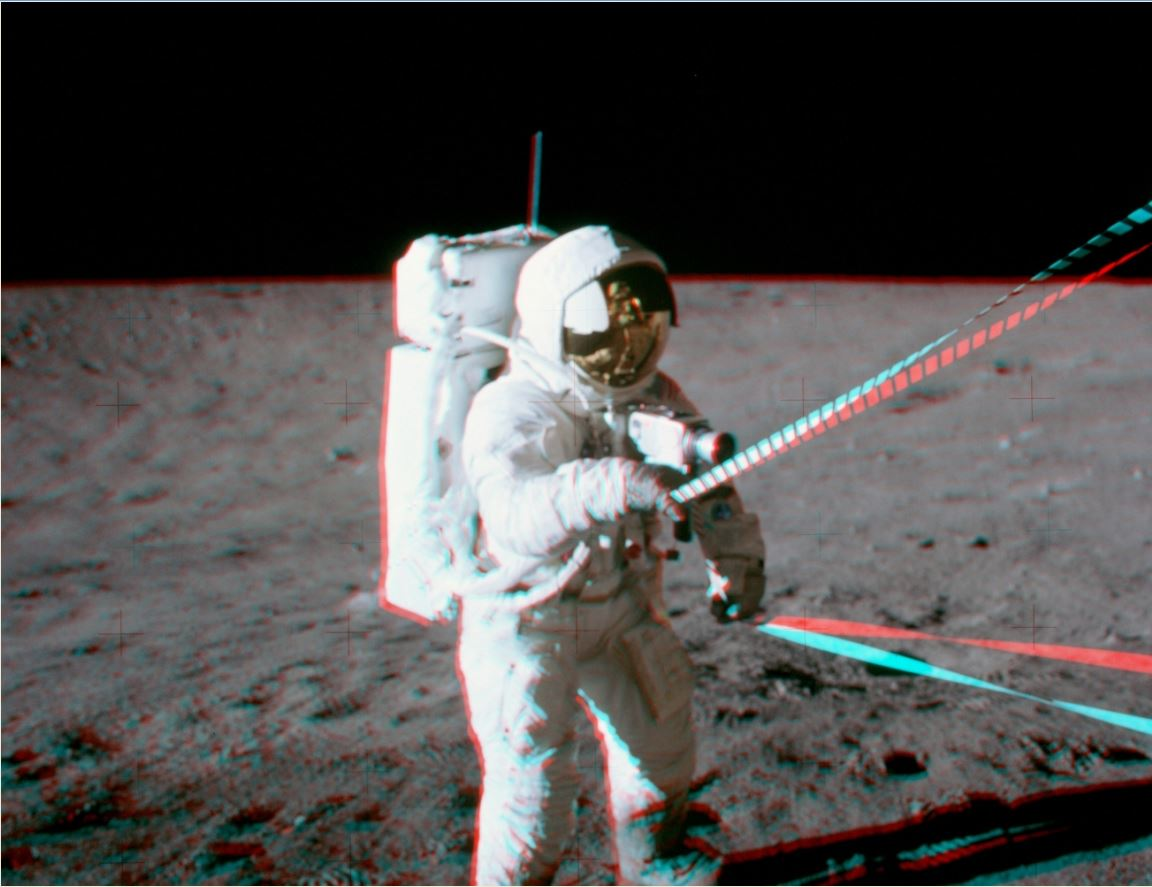
\includegraphics[width=0.7\textwidth]{daten/pics/astronaut1.jpg}
\end{figure}

\subsection{FILE 5:}
\label{sec:charlie_daten_5}

\begin{lstlisting}

Time Machine Prior Art:

Pub. No.:WO/2009/056125 International Application No.:PCT/DE2008/001787 Publication Date:07.05.2009 International Filing Date:28.10.2008


Pub. No.:		WO/2008/143237		International Application No.:		PCT/JP2008/059191
Publication Date:		27.11.2008		International Filing Date:		20.05.2008

Pub. No.:WO/2008/094611 International Application No.:PCT/US2008/001241 Publication Date:07.08.2008 International Filing Date:30.01.2008
PriorityData:
11/700,015		31.01.2007		US
Title: SIMULATION SYSTEM IMPLEMENTING REAL-TIME MACHINE DATA


\end{lstlisting}

\subsection{FILE 6:}
\label{sec:charlie_daten_6}

\begin{lstlisting}

Subject:
Instructions
From:
Charlie <charlie@m57.biz>
Date:
Fri, 04 Dec 2009 13:06:23 -0800
To:
jamie@project2400.com

J,

Got the deposit.  The password to get the info is nitro. Use the steg program we talked about.  And don't forget to delete these emails.

C

\end{lstlisting}

\subsection{FILE 7:}
\label{sec:charlie_daten_7}

\begin{lstlisting}

Subject:
I Found Something
From:
Charlie <charlie@m57.biz>
Date:
Fri, 04 Dec 2009 09:41:47 -0800
To:
andy@swexpert.com

Andy,

Lucky for me, I just happened to stumble across this.  I found a prior patent that will definitely invalidate your current immortality patent.  You should have used my boss's prior art services, but, oh well, I'll just use your negligence to benefit me.  I want 100k or I'll release this publicly.  I don't need to tell you how much this will hurt your business if I go public with this.  Don't involve the cops or this information will go public.  See the attachment for details on what I found.  I'll be in touch with my bank acct number.  The password for the zip file will be hidden in the next picture I send you.

C

\end{lstlisting}

\subsection{FILE 8:}
\label{sec:charlie_daten_8}

\begin{figure}[H]
	\centering
	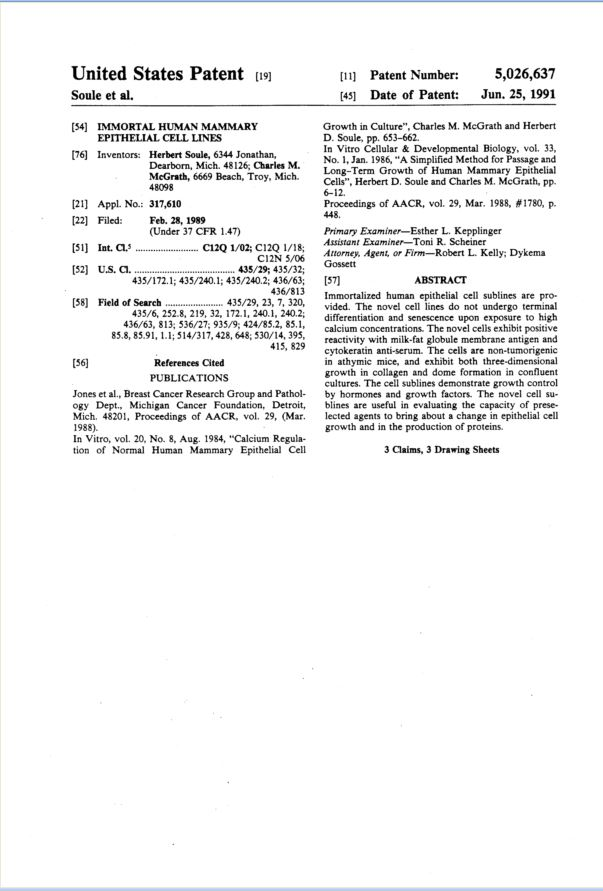
\includegraphics[width=0.7\textwidth]{daten/pics/patent1.jpg}
\end{figure}

\begin{figure}[H]
	\centering
	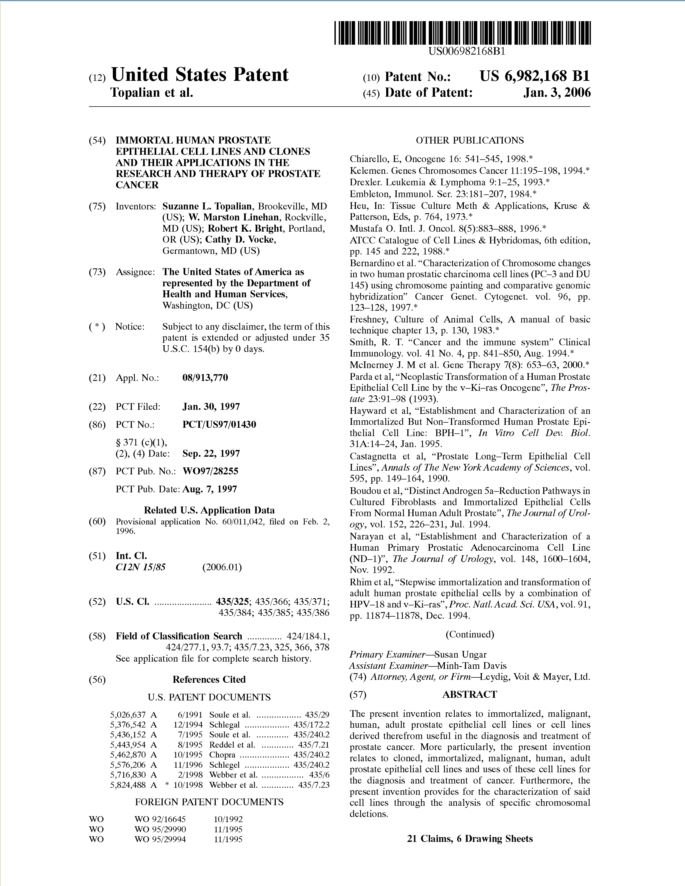
\includegraphics[width=0.7\textwidth]{daten/pics/patent2.jpg}
\end{figure}

\subsection{FILE 9:}
\label{sec:charlie_daten_9}

\begin{lstlisting}

Subject:
Picture
From:
Charlie <charlie@m57.biz>
Date:
Mon, 07 Dec 2009 11:44:18 -0800
To:
andy@swexpert.com

Andy,

Here's the picture I promised...  Make sure you delete this.

C

\end{lstlisting}

\subsection{FILE 10:}
\label{sec:charlie_daten_10}

\begin{figure}[H]
	\centering
	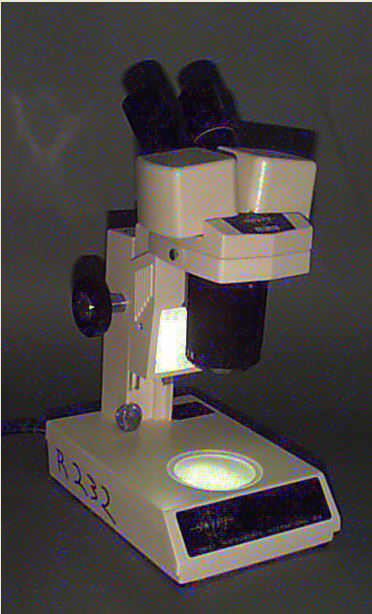
\includegraphics[width=0.5\textwidth]{daten/pics/microscope1.jpg}
\end{figure}
